\documentclass[a4paper, 11pt]{report}

\usepackage{amssymb, amstext, amsmath, amsthm, enumerate, float, graphicx, mathtools, csvsimple, bbm, calc, listings, textcomp, color}
\usepackage[margin = .55in, footskip = 20pt]{geometry}  %geometry package to set margins thin


\lstset{
  language=R,
  aboveskip={-10pt},
  backgroundcolor=\color{white},   		% choose the background color; you must add \usepackage{color} or \usepackage{xcolor}
  basicstyle=\tiny,        		% the size of the fonts that are used for the code
  breakatwhitespace=false,         		% sets if automatic breaks should only happen at whitespace
  breaklines=true,                		% sets automatic line breaking
  % caption=\lstname,                   	% show the filename of files included with \lstinputlisting; also try caption instead of title
  % captionpos=b,                    	% sets the caption-position to bottom
  columns=fixed,
  commentstyle=\color[rgb]{0.133,0.545,0.133},     			% comment style
  % commentstyle=\color{black}
  deletekeywords={hat,se},            	% if you want to delete keywords from the given language
  % escapeinside={\%*}{*)},          	% if you want to add LaTeX within your code
  extendedchars=true,              		% lets you use non-ASCII characters; for 8-bits encodings only, does not work with UTF-8
  firstnumber=1,						% start first number at 1 if importing multiple code files
  % frame=single,                    	% adds a frame around the code
  identifierstyle=\ttfamily\color[rgb]{0,0,0},
  keepspaces=true,                 		% keeps spaces in text, useful for keeping indentation of code (possibly needs columns=flexible)
  keywordstyle=\bfseries\ttfamily\color[rgb]{0,0,1},       	% keyword style
  % keywordstyle=\color{black},
  morekeywords={pdf,lty,lwd,col,xlim,ylim,xlab,ylab,type,main,head,header,TRUE,True,T,true,FALSE,F,False,false},            		% if you want to add more keywords to the set
  numbers=left,                    		% where to put the line-numbers; possible values are (none, left, right)
  numberfirstline=true,					% number the first line in your code file or not
  numbersep=5pt,                   		% how far the line-numbers are from the code
  numberstyle=\tiny\color[rgb]{0.5,0.5,0.5}, 				% the style that is used for the line-numbers
  % rulecolor=\color{black},         	% if not set, the frame-color may be changed on line-breaks within not-black text (e.g. comments (green here))
  showspaces=false,                		% show spaces everywhere adding particular underscores; it overrides 'showstringspaces'
  showstringspaces=false,          		% underline spaces within strings only
  showtabs=false,                  		% show tabs within strings adding particular underscores
  stepnumber=5,                    		% the step between two line-numbers. If it's 1, each line will be numbered 
  stringstyle=\ttfamily\color[rgb]{0.627,0.126,0.941},     	% string literal style
  % stringstyle=\bfseries\ttfamily\color[rgb]{0.5,0,0.5},       	% keyword style
  % stringstyle=\color{black},								  % string literal style
  tabsize=3,                       		% sets default tabsize to 2 spaces
  title=\lstname,                   	% show the filename of files included with \lstinputlisting; also try caption instead of title
  upquote=true,
  xleftmargin=.15in,						% indent the left margin including line numbers and code  
  literate=									% colors numbers but the * makes it only color outside comments and strings
    *{0}{{{\color[rgb]{0.95,0.25,0}0}}}1
    {1}{{{\color[rgb]{0.95,0.25,0}1}}}1
    {2}{{{\color[rgb]{0.95,0.25,0}2}}}1
    {3}{{{\color[rgb]{0.95,0.25,0}3}}}1
    {4}{{{\color[rgb]{0.95,0.25,0}4}}}1
    {5}{{{\color[rgb]{0.95,0.25,0}5}}}1
    {6}{{{\color[rgb]{0.95,0.25,0}6}}}1
    {7}{{{\color[rgb]{0.95,0.25,0}7}}}1
    {8}{{{\color[rgb]{0.95,0.25,0}8}}}1
    {9}{{{\color[rgb]{0.95,0.25,0}9}}}1
}

\newcommand{\tab}{\hspace*{1.0em}} % multiple of width of a capital M
\newcommand{\imply}{\tab \Longrightarrow \tab}


\begin{document}

	\begin{titlepage}
	\newgeometry{margin = 0.75in}
	\vspace*{1.5in}
	\noindent\rule{\textwidth}{1pt}
	\begin{flushright}
		\LARGE \textbf{Michael Bissell} \\ \vspace{0.5in}
		\Large STA 250 \\
		\large \textit{Advanced Statistical Computing} \\ \vspace{0.5in}
		\Large Assignment 4 \\
			GPU Computing
	\end{flushright}
	\noindent\rule{\textwidth}{1pt}
	\end{titlepage}
	\restoregeometry


%	\vspace*{-.2in}
%	\hrule
%	\begin{center}
%		\LARGE
%		\textbf{Michael Bissell} \\
%		\Large
%		STA 250 Homework 2 \\
%		Code Swap Review 	
%	\end{center}
%	\vspace{-.2in}
%	\noindent\rule{\textwidth}{1pt} \\ 
	

	\noindent\rule{\textwidth}{1pt} \\
	
	\vspace{-7pt}
	\noindent
	1) Implement a kernel to obtain samples from a truncated normal random variable 
	\begin{enumerate}[a)] %\setlength\itemindent{0.2em}
		\item Write a kernel in CUDA C to obtain samples from a truncated normal random variable of the form: 
			$$ X \sim TN(\mu,\sigma^2;(a,b)) \equiv N(\mu,\sigma^2)1_{ \{ X \in (a,b) \} }$$ 
			
			\noindent \textit{Answer:} See code appendices at end of report.

		\item Compile your CUDA kernel using nvcc and check it can be launched properly 
		
			\noindent \textit{Answer:} If only I could count the number of times I had to compile and re-compile this kernel...  See below.
			
		\item Sample 10,000 random variables from TN(2,1;(0,1.5)), and verify the expected value (roughly) matches the theoretical value (see class notes 
			for details). 
			
			\noindent \textit{Answer:} From the class notes, Lecture 13, if $W \sim TN(\mu,\sigma;(a,b))$, then the expected value of $W$ is: 
				$$ \mathbb{E}[W] = \mu + \sigma \frac{ \phi\left( \frac{a-\mu}{\sigma}\right) - \phi\left( \frac{b-\mu}{\sigma}\right) }{ \Phi\left( \frac{b-\mu}{\sigma}\right) - \Phi\left( \frac{a-\mu}{\sigma}\right) } = 0.9570.$$
				The observed mean from the 10,000 samples is 0.958, which is extremely close to the theoretical value and the density plots virtually completely overlap when plotted as vertical lines, as shown in Figure \ref{density-1c} below.
				\vspace*{-12pt}
				\begin{figure}[H]
					\centering
					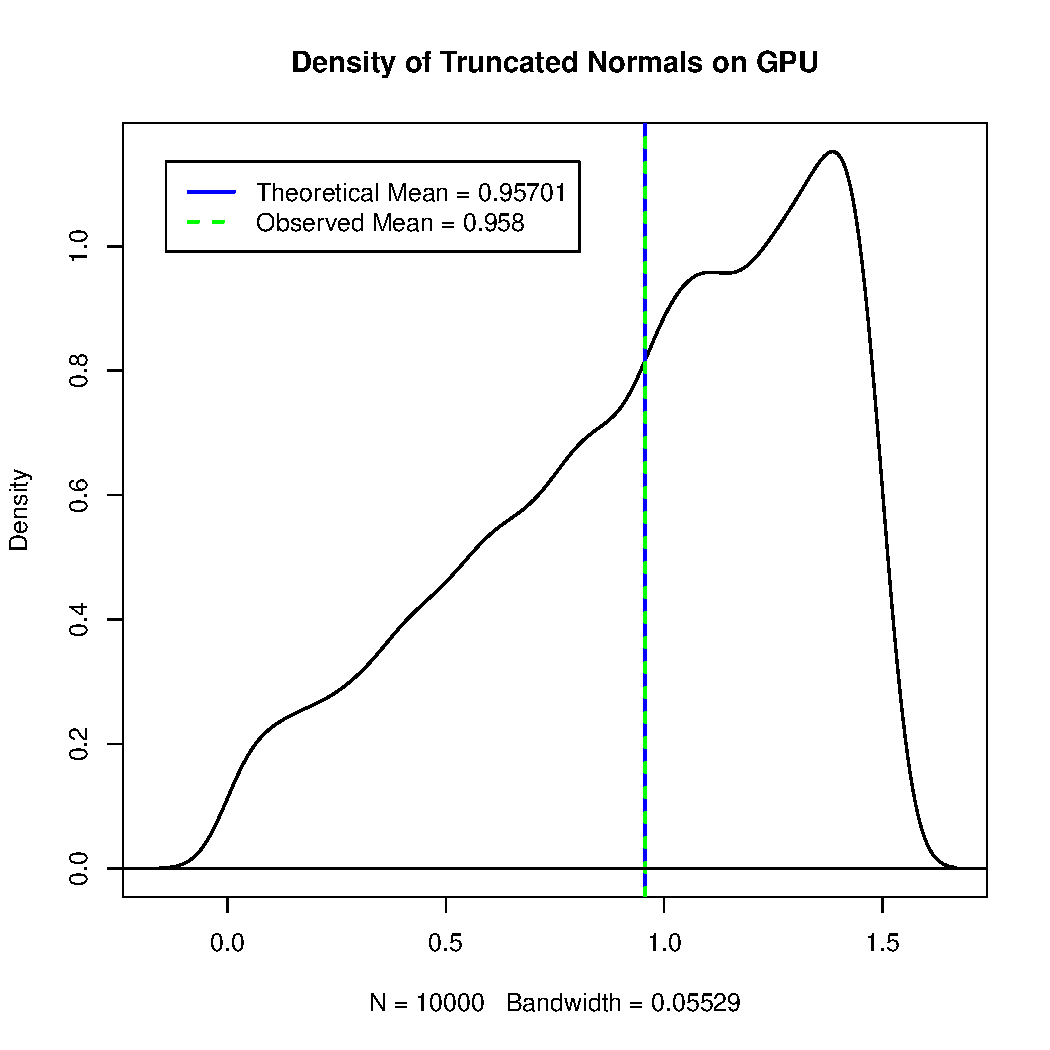
\includegraphics[scale=0.55]{density-1c.pdf}
					\caption{Density Plot of 10,000 Truncated Normals}
					\label{density-1c}
				\end{figure}				
				
			
		\item Write an R function for sampling truncated normal random variables (possibly using a different algorithm). You may also use the code provide 
			in the GitHub repo. Sample 10,000 random variables from this function and verify the mean (roughly) matches the theoretical values. 
			
			\noindent \textit{Answer:} We simply use rtruncnorm() function in the R package truncnorm. The observed mean from the 10,000 samples is 0.94819, which is extremely close to the theoretical value of 0.95701 and the density plots virtually completely overlap when plotted as vertical lines, as shown in Figure \ref{density-1d} below.
				\begin{figure}[H]
					\centering
					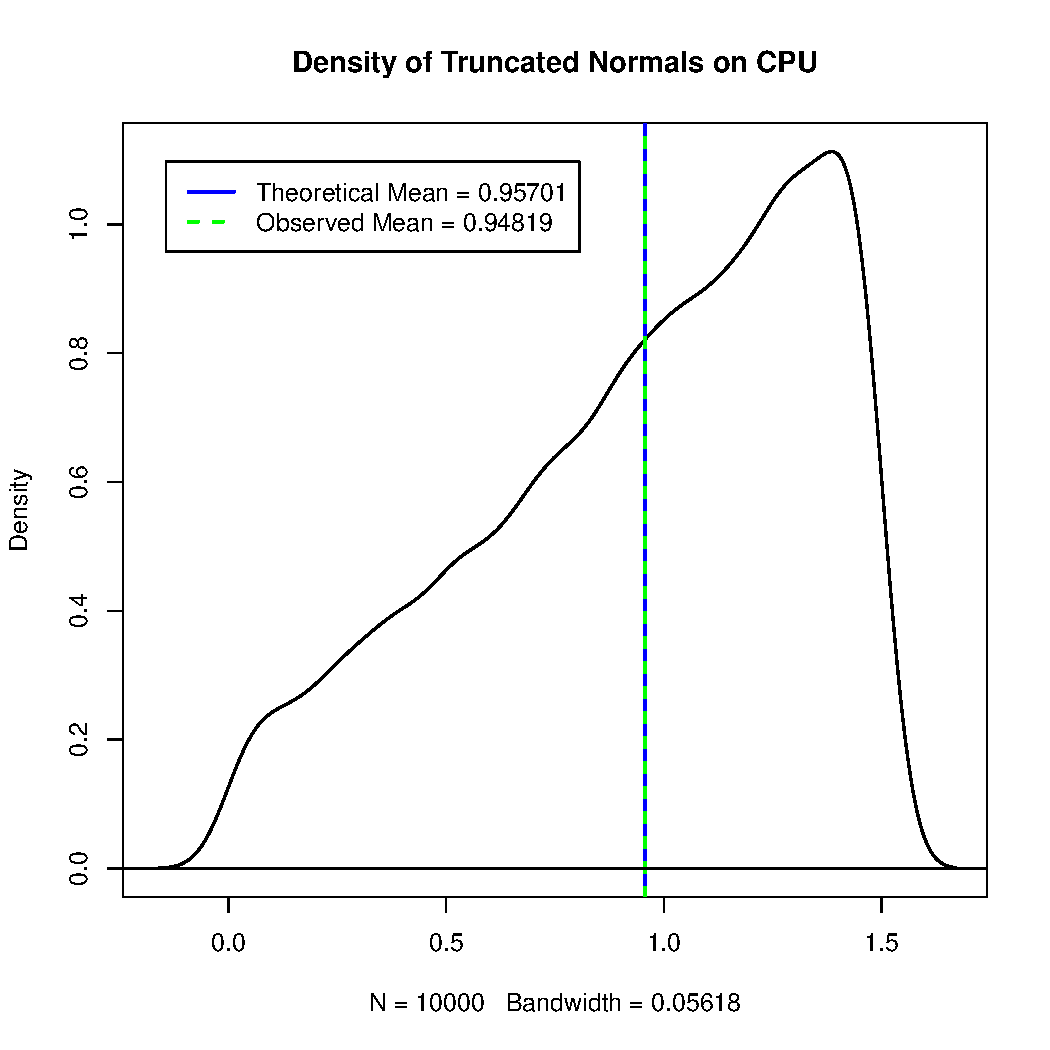
\includegraphics[scale=0.55]{density-1d.pdf}
					\caption{Density Plot of 10,000 Truncated Normals}
					\label{density-1d}
				\end{figure}
			
		\item Time your RCUDA function and pure R function for $n=10^k$ for $k=1,2,\ldots,8$. Plot the total runtimes for both functions on the y-axis as 
			a function of n (on the log-scale as the x-axis). At what point did/do you expect the GPU function to outperform the non-GPU function? You may also want to decompose the GPU runtimes into copy to/kernel/copy back times for further detailed analysis.
			
			\noindent \textit{Answer:} 
				\begin{figure}[H]
					\centering
					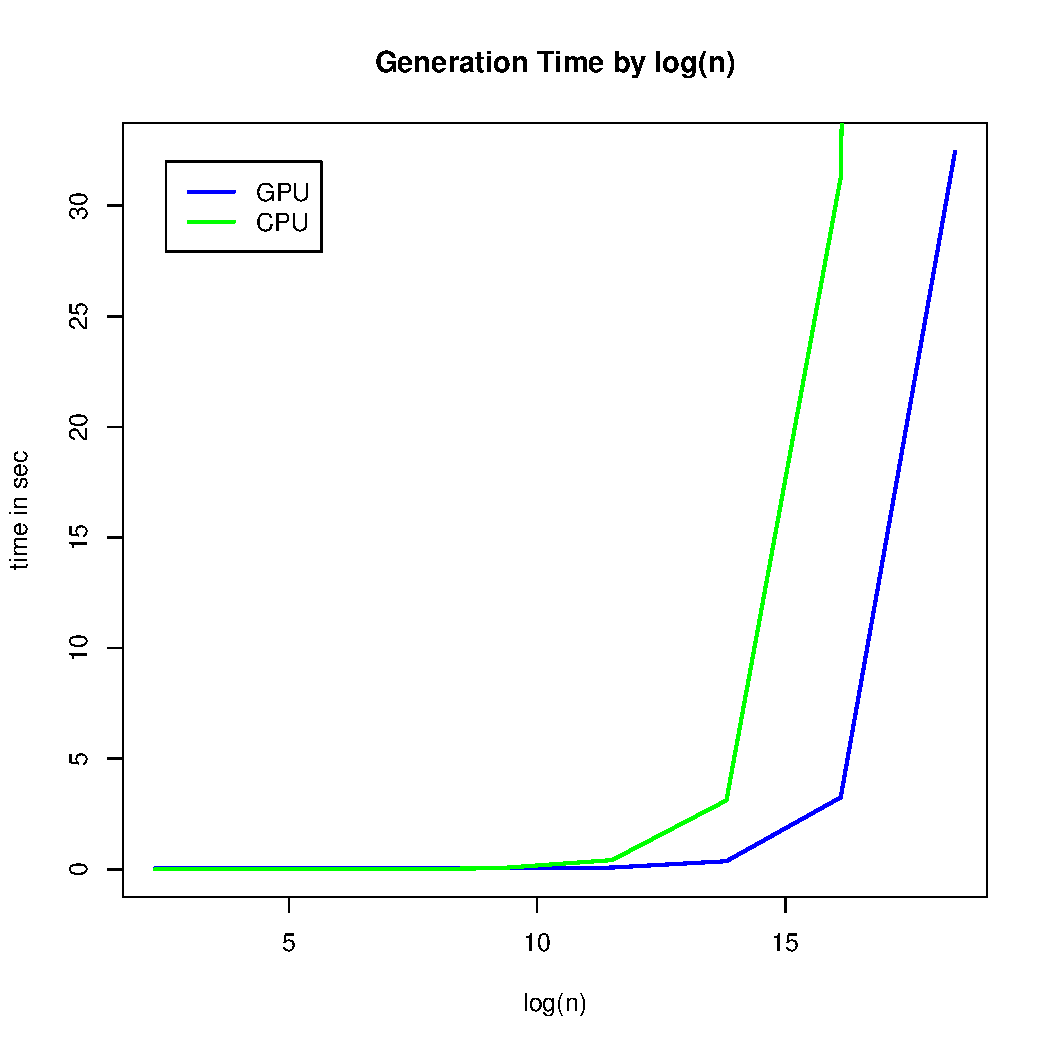
\includegraphics[scale=0.55]{plot-1e.pdf}
					\caption{Generation Time by log(n)}
					\label{plot-1e}
				\end{figure}
				\begin{table}[H]
				\centering
				\begin{tabular}{rrrrr}
				  \hline
				 & n & copyToDevice & kernel & copyFromDevice \\ 
				  \hline
				1 & 10 & 0.00 & 0.04 & 0.00 \\ 
				  2 & 100 & 0.00 & 0.05 & 0.00 \\ 
				  3 & 1000 & 0.00 & 0.04 & 0.00 \\ 
				  4 & 10000 & 0.00 & 0.05 & 0.00 \\ 
				  5 & 100000 & 0.01 & 0.08 & 0.00 \\ 
				  6 & 1000000 & 0.03 & 0.33 & 0.01 \\ 
				  7 & 10000000 & 0.26 & 2.92 & 0.07 \\ 
				  8 & 100000000 & 2.64 & 29.15 & 0.66 \\ 
				   \hline
				\end{tabular}
				\end{table}
				
		\item Verify that both your GPU and CPU code work for $a=-\infty \text{ and/or } b=+\infty$.
			
			\noindent \textit{Answer:} We use $N(0,1) = TN(0,1;(-\infty, \infty))$, where we directly initialize the vectors `lo' and `hi' with values `-Inf' and `Inf', which are correctly handled by R and RCUDA.  The theoretical mean is obviously zero by symmetry and the observed mean from the 10,000 samples is -0.00147, which is extremely close and the density plots virtually completely overlap when plotted as vertical lines, as shown in Figure \ref{density-1f} below.  This along with part g) below, demonstrates that the code *appears* to works correctly.
				\vspace*{-12pt}
				\begin{figure}[H]
					\centering
					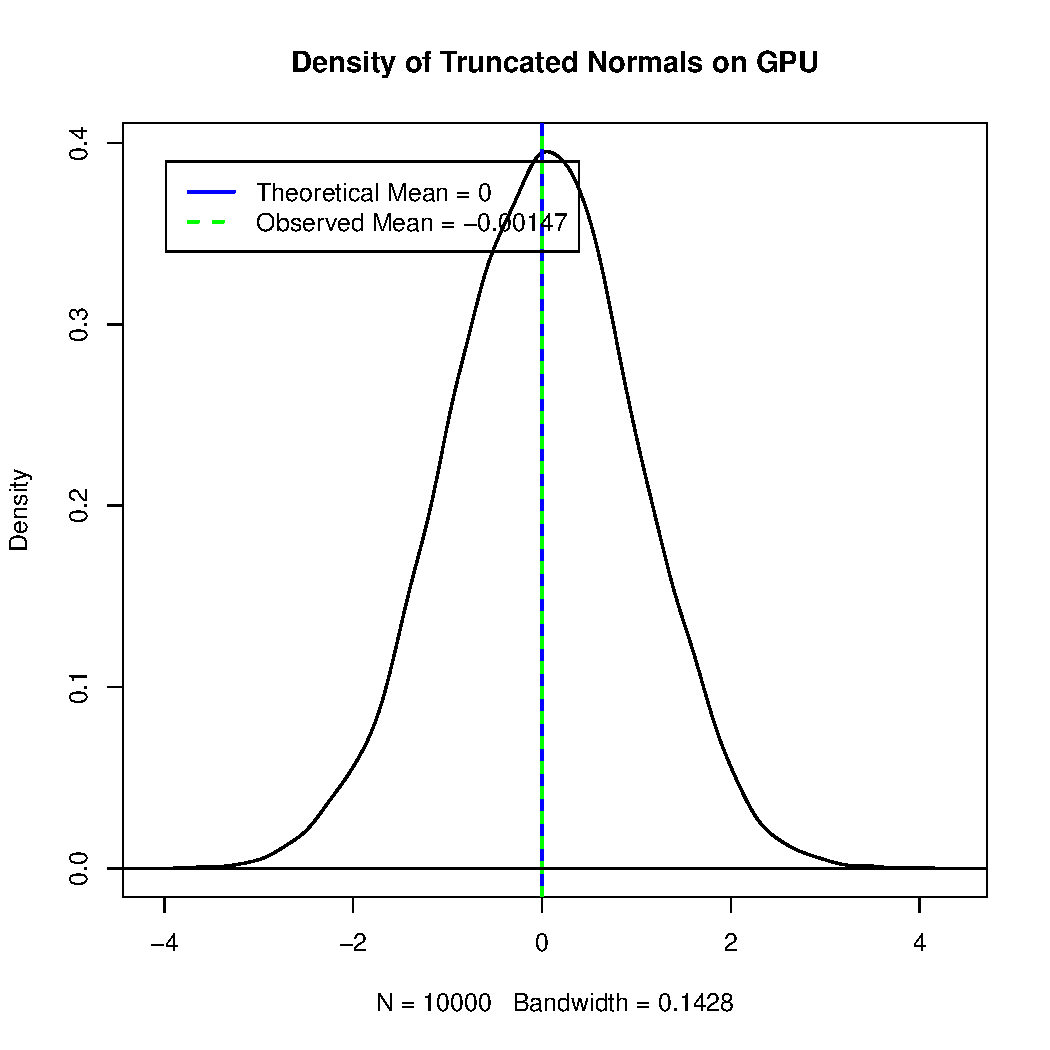
\includegraphics[scale=0.5]{density-1f.pdf}
					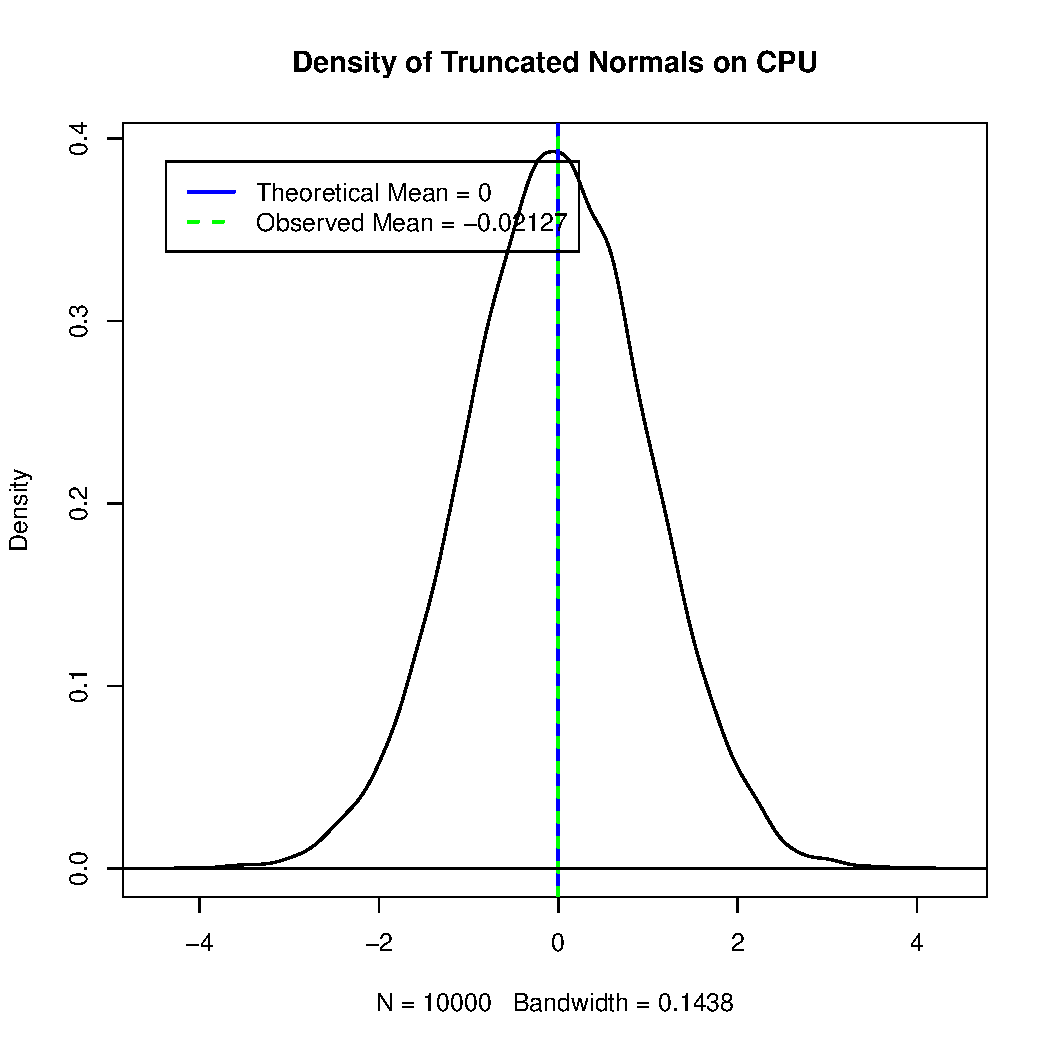
\includegraphics[scale=0.5]{density-1f-cpu.pdf}
					\caption{Density Plot of 10,000 Truncated Normals on GPU and CPU}
					\label{density-1f}
				\end{figure}
			
		\item Verify that both your GPU and CPU code work for truncation regions in the tail of the distribution e.g., $a=-\infty,b=-10,\mu=0,\sigma=1$.
			
			\noindent \textit{Answer:} From the class notes, Lecture 13, if $U \sim TN(\mu,\sigma;(-\infty,b))$, then the expected value of $U$ is: 
				$$ \mathbb{E}[U] = \mu - \sigma \frac{ \phi\left( \frac{b-\mu}{\sigma}\right) }{ \Phi\left( \frac{b-\mu}{\sigma}\right) } = -10.09809.$$
				The observed mean from the 10,000 samples is −10.1, which is extremely close to the theoretical value and the density plots virtually completely overlap when plotted as vertical lines, as shown in Figure \ref{density-1g} below.
				\vspace*{-12pt}
				\begin{figure}[H]
					\centering
					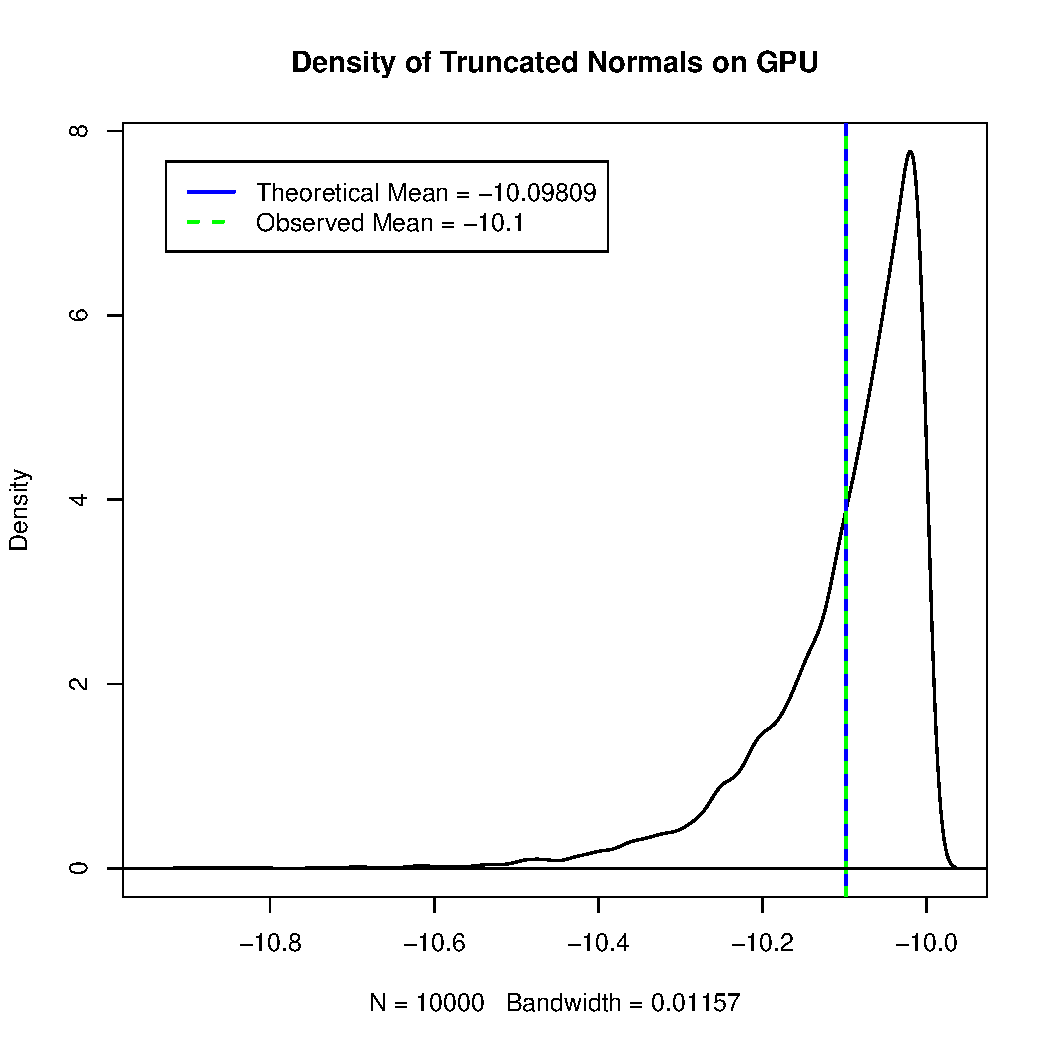
\includegraphics[scale=0.5]{density-1g.pdf}
					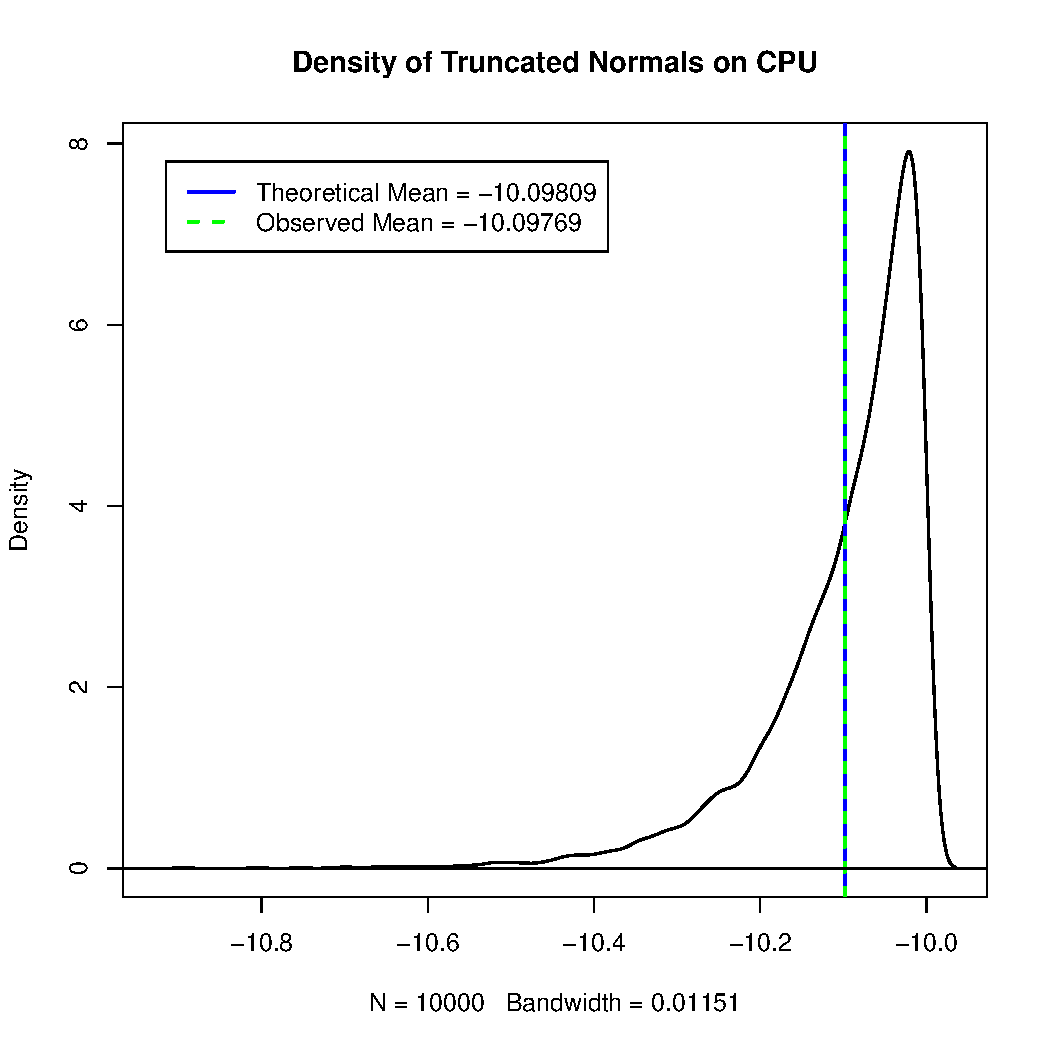
\includegraphics[scale=0.5]{density-1g-cpu.pdf}
					\caption{Density Plot of 10,000 Truncated Normals on GPU and CPU}
					\label{density-1g}
				\end{figure}	
		
			
	\end{enumerate}
	\noindent\rule{\textwidth}{1pt} \\ \\ \noindent
	2) In this question you will implement Probit MCMC i.e., fitting a Bayesian Probit regression model using MCMC. This model turns out to be  computationally nice and simple, lending itself to a Gibbs sampling algorithm with each distribution available in sample-able form. The model is as follows:
	$$ Y_i \vert Z_i \sim 1_{\{Z_i>0\}}$$
	$$ Z_i|\beta \sim N(x_i^T\beta,1)$$
	$$ \beta \sim N(\beta_0,\Sigma_0),$$
	where $\beta_0$ is a $p\times1$ vector corresponding to the prior mean, and $\Sigma_0^{-1}$ is the prior precision matrix. Note that for convenience we supply $\Sigma_0^{-1}$ as an argument to the probit MCMC function, to allow for flat priors for $\beta$.  \\
	
	\noindent\textit{Answer:} What we want are the estimates of $\beta$'s and thus we derive the posterior distribution of the $\beta$'s and take their means as the estimates.  We have:
	$$ \pi(\beta) \propto \exp\left\lbrace -\frac{1}{2}\left(\beta-\beta_0\right)^T\Sigma_0^{-1}\left(\beta-\beta_0\right)   \right\rbrace$$
	$$ p(\vec{z} \vert x_i,\beta) \propto \prod_{i=1}^{n}p(z_i \vert x_i, \beta) \propto \exp\left\lbrace -\frac{1}{2}\sum_{i=1}^{n}\left(z_i -				
		x_i^T\beta \right)^2 \right\rbrace \propto p(Z \vert X,\beta) \propto \exp\left\lbrace -\frac{1}{2}\left(Z-X\beta \right)^2 \right\rbrace$$
	$$ p(Z \vert X,Y,\beta) \sim \begin{cases} 	TN_p(X\beta,I_p;[0,\infty)) & y = 1 \\  TN_p(X\beta,I_p;(-\infty,0]) & y = 0 \end{cases}$$
	Thus to get estimates of our parameters $\beta$ given the data, we find the posterior distribution of $\beta | X,Y,Z$ as follows:
	$$ p(\beta \vert X,Y,Z) \propto \pi(\beta)p(Z \vert X,Y,\beta) \propto \exp\left\lbrace -\frac{1}{2}\left[\left(\beta-\beta_0\right)^T\Sigma_0^{-1}\left(\beta-\beta_0\right) + \left(Z-X\beta \right)^2 \right]  \right\rbrace $$
	\begin{flalign*} 
		& \propto \exp\left\lbrace -\frac{1}{2}\left[\left(\beta-\beta_0\right)^T\Sigma_0^{-1}\left(\beta-\beta_0\right) + \left(Z-X\beta \right)^T\left(Z-X\beta \right) \right]  \right\rbrace 	\\
		& \propto \exp\left\lbrace -\frac{1}{2}\left[\beta^T\Sigma_0^{-1}\beta - \beta^T\Sigma_0^{-1}\beta_0 - \beta_0^T\Sigma_0^{-1}\beta    + \beta_0^T\Sigma_0^{-1}\beta_0 + Z^TZ - Z^TX\beta - \beta^TX^TZ + \beta^TX^TX\beta \right]  \right\rbrace \\
		& \propto \exp\left\lbrace -\frac{1}{2}\left[\beta^T\Sigma_0^{-1}\beta - \beta^T\Sigma_0^{-1}\beta_0 - \beta_0^T\Sigma_0^{-1}\beta  - Z^TX\beta - \beta^TX^TZ + \beta^TX^TX\beta \right]  \right\rbrace \\
		& \propto \exp\left\lbrace -\frac{1}{2}\left[\beta^T\left(\Sigma_0^{-1} + X^TX\right)\beta - \beta^T\left(\Sigma_0^{-1}\beta_0 + X^TZ\right) - \left(\beta_0^T\Sigma_0^{-1} + Z^TX\right)\beta  \right]  \right\rbrace	\\
		& \text{From here we can identify the posterior multivariate normal mean and variance by comparing to} \\
		& \text{standard quadratic forms.  For a standard quadratic form, we would have:}	\\
		& \propto \exp\left\lbrace -\frac{1}{2}\left[\left(X-\mu\right)^T\Sigma^{-1}\left(X-\mu\right)\right]  \right\rbrace 
		\propto \exp\left\lbrace -\frac{1}{2}\left[X^T\Sigma^{-1}X - X^T\Sigma^{-1}\mu - \mu^T\Sigma^{-1}X + \mu^T\Sigma^{-1}\mu\right]\right\rbrace \\
		& \text{By equating the first term in the posterior derivation above and the first term in the standard } \\
		& \text{form above, we identify } X^T\Sigma^{-1}X = \beta^T\left(\Sigma_0^{-1} + X^TX\right)\beta \text{.  Thus the posterior variance is } \\
		& \left(\Sigma_0^{-1} + X^TX\right) \text{. Similarly, equating the second terms, we see that } X^T\Sigma^{-1}\mu = \beta^T\left(\Sigma_0^{-1} + X^TX\right)  \\
		& \text{giving } \Sigma^{-1}\mu = \left(\Sigma_0^{-1} + X^TX\right) \imply \left(\Sigma_0^{-1} + X^TX\right) \mu = \left(\Sigma_0^{-1} + X^TX\right) \\
		& \imply \mu = \left(\Sigma_0^{-1} + X^TX\right)^{-1}\left(\Sigma_0^{-1}\beta_0 + X^TZ\right) \\
		& \text{Thus we have:} 
	\end{flalign*}
	$$ p(\beta \vert X,Y,Z) \propto N_p\left( \quad  \left(\Sigma_0^{-1} + X^TX\right)^{-1}\left(\Sigma_0^{-1}\beta_0 + X^TZ\right) \quad , \quad \left(\Sigma_0^{-1} + X^TX\right) \quad \right) $$
 
	
	
	\begin{enumerate}[a)] \setlength\itemindent{0.2em} 
		\item Write a R function `probit\_mcmc' to sample from the posterior distribution of $\beta$ using the CPU only.  Your function should return the posterior samples of $\beta$ as a matrix/array or `mcmc' object (if using R). The posterior samples of Z do not need to be returned (and should not be stored -- they will take up too much memory!). 
		
		\textit{Answer:} See code appendix for ``probit\_mcmc\_cpu'' below and results from problems below.
		
		\item Write a RCUDA function `probit\_mcmc' to sample from the posterior distribution of $\beta$ using the CPU and GPU.  You can also compute the block and grid dimensions within your function if preferred. Note that the GPU should only be used for the sampling of the $Z_i$ vector. Your function should return the posterior samples of $\beta$ as a matrix/array or `mcmc' object (if using R). The posterior samples of Z do not need to be returned (and should not be stored -- they will take up too much memory!).
		
		\textit{Answer:} See code appendix for ``probit\_mcmc\_gpu'' below and results from problems below.
		
		\item Test your code by fitting the mini dataset `mini\_test.txt'. This dataset can be generated by running the file `sim\_probit.R', supplied in the course GitHub repo. The first column of the dataset corresponds to `y', with all other columns corresponding to `X'. Assume prior parameters $\beta_0=\vec{0}$ and $\Sigma_0^{-1}=\mathbf{0}$. Verify that both functions give posterior means/medians that are at least relatively close to the true values (in `mini\_pars.txt', also generated when you run `sim\_probit.R') and the estimates produced by standard GLM functions.
		
			\textit{Answer:} We can see that the GPU runtime is considerably longer than the CPU runtime as expected when the copyToDevice overhead is not offset by the speed of the GPU since the number of threads in the mini dataset is so small and the $\beta$'s are all over the place for the CPU but roughly on the correct scale for the GPU:
				\begin{table}[H]
				\centering
				\begin{tabular}{rlrrrrr}
				  \hline
				 & X & user.self & sys.self & elapsed & user.child & sys.child \\ 
				  \hline
				1 & gpu\_time & 103.98 & 3.12 & 107.07 &   0 &   0 \\ 
				  2 & cpu\_time & 1.68 & 0.00 & 1.68 &   0 &   0 \\ 
				   \hline
				\end{tabular}
				\end{table}
				\begin{table}[H]
				\centering
				\begin{tabular}{rlrrrrrrrr}
				  \hline
				 & Source & Beta0 & Beta1 & Beta2 & Beta3 & Beta4 & Beta5 & Beta6 & Beta6 \\ 
				  \hline
				1 & GPU & 17.73 & 5.00 & -66.90 & -3.05 & 27.17 & -0.66 & 21.85 & -6.87 \\ 
				  2 & CPU & 1.62 & 0.47 & -5.50 & -0.02 & 2.25 & -0.08 & 2.05 & -0.31 \\ 
				  3 & PARS & 0.57 & -0.11 & -2.06 & 0.12 & 1.05 & -0.10 & 1.23 & -0.03 \\ 
				   \hline
				\end{tabular}
				\end{table}
		
		
		\item Run `sim\_probit.R' to create each of the following datasets. Then analyze as many as possible, using both your CPU and GPU code:
		
		    `data\_01.txt': n=1000 for `niter=2000', `burnin=500' 
			\begin{table}[H]
			\centering
			\begin{tabular}{rlrrrrr}
			  \hline
			 & X & user.self & sys.self & elapsed & user.child & sys.child \\ 
			  \hline
			1 & gpu\_time & 103.62 & 1.71 & 105.34 &   0 &   0 \\ 
			  2 & cpu\_time & 3.57 & 0.00 & 3.57 &   0 &   0 \\ 
			   \hline
			\end{tabular}
			\end{table}
			\begin{table}[H]
			\centering
			\begin{tabular}{rlrrrrrrrr}
			  \hline
			 & Source & Beta0 & Beta1 & Beta2 & Beta3 & Beta4 & Beta5 & Beta6 & Beta6 \\ 
			  \hline
			1 & GPU & -0.05 & -0.91 & 0.19 & 1.75 & 1.71 & -1.18 & 2.30 & 0.74 \\ 
			  2 & CPU & 0.17 & -1.01 & 0.38 & 2.19 & 1.73 & -1.03 & 2.53 & 0.87 \\ 
			  3 & PARS & 0.14 & -0.97 & 0.31 & 1.87 & 1.49 & -0.95 & 2.42 & 0.80 \\ 
			   \hline
			\end{tabular}
			\end{table}
			
		    `data\_02.txt': n=10000 for `niter=2000', `burnin=500' 
			\begin{table}[H]
			\centering
			\begin{tabular}{rlrrrrr}
			  \hline
			 & X & user.self & sys.self & elapsed & user.child & sys.child \\ 
			  \hline
			1 & gpu\_time & 115.88 & 4.31 & 120.20 &   0 &   0 \\ 
			  2 & cpu\_time & 24.04 & 0.00 & 24.05 &   0 &   0 \\ 
			   \hline
			\end{tabular}
			\end{table}
			\begin{table}[H]
			\centering
			\begin{tabular}{rlrrrrrrrr}
			  \hline
			 & Source & Beta0 & Beta1 & Beta2 & Beta3 & Beta4 & Beta5 & Beta6 & Beta6 \\ 
			  \hline
			1 & GPU & 0.12 & 0.17 & -0.65 & 0.12 & 1.20 & 0.31 & 0.57 & -0.49 \\ 
			  2 & CPU & 0.11 & 0.13 & -0.58 & 0.11 & 1.10 & 0.28 & 0.49 & -0.45 \\ 
			  3 & PARS & 0.09 & 0.16 & -0.58 & 0.12 & 1.10 & 0.27 & 0.48 & -0.44 \\ 
			   \hline
			\end{tabular}
			\end{table}
			
		    `data\_03.txt': n=100000 for `niter=2000', `burnin=500' 
			\begin{table}[H]
			\centering
			\begin{tabular}{rlrrrrr}
			  \hline
			 & X & user.self & sys.self & elapsed & user.child & sys.child \\ 
			  \hline
			1 & gpu\_time & 181.76 & 28.61 & 210.37 &   0 &   0 \\ 
			  2 & cpu\_time & 211.76 & 0.06 & 211.81 &   0 &   0 \\ 
			   \hline
			\end{tabular}
			\end{table}
			\begin{table}[H]
			\centering
			\begin{tabular}{rlrrrrrrrr}
			  \hline
			 & Source & Beta0 & Beta1 & Beta2 & Beta3 & Beta4 & Beta5 & Beta6 & Beta6 \\ 
			  \hline
			1 & GPU & 2.44 & 1.38 & 0.39 & -0.16 & -0.69 & -1.33 & 0.44 & -1.31 \\ 
			  2 & CPU & 2.45 & 1.37 & 0.42 & -0.16 & -0.69 & -1.34 & 0.45 & -1.33 \\ 
			  3 & PARS & 2.45 & 1.38 & 0.41 & -0.15 & -0.69 & -1.33 & 0.45 & -1.35 \\ 
			   \hline
			\end{tabular}
			\end{table}
			
		    `data\_04.txt': n=1000000 for `niter=2000', `burnin=500'
		    \begin{table}[H]
		    \centering
		    \begin{tabular}{rlrrrrr}
		      \hline
		     & X & user.self & sys.self & elapsed & user.child & sys.child \\ 
		      \hline
		    1 & gpu\_time & 792.26 & 283.64 & 1075.87 &   0 &   0 \\ 
		      2 & cpu\_time & 2147.28 & 36.90 & 2184.05 &   0 &   0 \\ 
		       \hline
		    \end{tabular}
		    \end{table}
		    \begin{table}[H]
		    \centering
		    \begin{tabular}{rlrrrrrrrr}
		      \hline
		     & Source & Beta0 & Beta1 & Beta2 & Beta3 & Beta4 & Beta5 & Beta6 & Beta6 \\ 
		      \hline
		    1 & GPU & -1.21 & 0.23 & 0.30 & 1.02 & 1.18 & 1.79 & 1.22 & -2.87 \\ 
		      2 & CPU & -1.21 & 0.23 & 0.30 & 1.01 & 1.18 & 1.78 & 1.22 & -2.87 \\ 
		      3 & PARS & -1.21 & 0.24 & 0.30 & 1.01 & 1.18 & 1.78 & 1.22 & -2.87 \\ 
		       \hline
		    \end{tabular}
		    \end{table}
		    
		    `data\_05.txt': n=10000000 for `niter=2000', `burnin=500' \\
		    data\_05.txt did actually complete for me after several runs of fixing bugs with a total runtime of approximately 4 hours for the GPU and 7.5 hours for the CPU.  However, while attempting to run these jobs in the background on AWS using an `\&', I introduced one final mistake in the write.csv step of the output, so I have no proof other than my word.
		    
		    We notice that the GPU code has overhead from copyToDevice that dominates runtime until the speed of multiple threads can overtake the copy time.  By looking at data\_03.txt, it seems that the break even point maybe in the neighborhood of 100,000 threads, after which, the GPU code creams the CPU code.  As seen in data\_04.txt, the runtime for the CPU is approxiately twice as long as the GPU code.
		    
		\item Discuss the relative performance of your CPU and GPU code. At what point do you think your GPU code would become competitive with the CPU code?
		
			\textit{Answer:} The first thing we notice is that the GPU code has overhead from copyToDevice that dominates runtime until the speed of multiple threads can overtake the copy time.  By looking at data\_03.txt, it seems that the break even point maybe in the neighborhood of 100,000 threads.  In additona, as noted in the assignment, ``the number of iterations used here is not sufficient to obtain reliable posterior estimates. This exercise is for illustration and learning purposes.''
			
			Additonally, we notice that the GPU estimates themselves seem to be a bit off for small datasets relative to built-in R functions.  This could indicate that there is a bug in our code, or perhaps the built-in R function is more efficient or accurate in computation.  As the size of the datasets increase, both estimates from the GPU and the CPU match very closely to the true parameter values.
			
			Lastly, as noted in the assignment, ``the number of iterations used here is not sufficient to obtain reliable posterior estimates. This exercise is for illustration and learning purposes.''
		
	\end{enumerate}


	
	%%%%%%%%%%%%%%%%%%%%%%%%
	% Code appendix
	%%%%%%%%%%%%%%%%%%%%%%%%
	\newpage
	
	\noindent\rule{\textwidth}{1pt} 
	\begin{center} 
		Code Appendix
	\end{center}
	\vspace*{-7pt}
	\noindent\rule{\textwidth}{1pt} \\
	\lstinputlisting{"rtruncnorm.cu"}
	\noindent\rule{\textwidth}{1pt} \\
	\lstinputlisting{"rtruncnorm_driver.R"}
	\noindent\rule{\textwidth}{1pt} \\
	\lstinputlisting{"probit_mcmc_driver.R"}
	\noindent\rule{\textwidth}{1pt} \\
	\lstinputlisting{"rtruncnorm_timer.R"}
	\noindent\rule{\textwidth}{1pt} \\	
\end{document}